\documentclass{IEEEtran}

\hbadness=99999

% Packages
\usepackage{amsmath}
\usepackage{physics}
\usepackage[cmintegrals]{newtxmath}
\usepackage{graphicx}
\usepackage{xurl} % Makes urls better
\graphicspath{{./images}}

% Title Stuff
\title{Engineering breakdown voltage in a pn-junction diode}
\author{Chase A. Lotito, \textit{SIUC Undergraduate}}
\date{}

% Makes a header!
\markboth{ECE447 --- Semiconductor Devices --- Project 3, April 2024}{Shell \MakeLowercase{\text
it{et al.}}: A Novel Tin Can Link}

\begin{document}

\maketitle % Makes the title

% ABSTRACT
\begin{abstract}
    % [A brief statement on what you plan to do in this project.]
For this lab, the goal is to design a one-sided abrupt silicon pn-junction diode. This diode must have a breakdown voltage of at least 60V with a forward-bias current of 50mA when applying 0.625V. We know that the minority carrier lifetimes are \(\tau_0 = 2 \times 10^{-7} s\). The parameters to engineer are doping density and cross-sectional area.
\end{abstract}

\section*{Introduction}

For this pn-junction experiment, the \textit{PN Junction Lab} from nanoHUB.org was used \cite{sim}.

\section*{Part I: Analytical Design}

Since we are using silicon, \(\mu_n = 1350 ~ \text{cm}^2/\text{Vs}\) and \(\mu_p = 480 ~ \text{cm}^2/\text{Vs}\). And, I assume \(T=300 ~ \text{K}\).

Using the Shockley diode equation, we can back-solve for the reverse saturation current \(I_s\) in our diode:

\begin{align*}
    I_D &= I_s(e^{V_D/V_{th}} - 1) \\
    \implies I_s &= I_D(e^{V_D/V_{th}} - 1)^{-1} \\
    &= (0.050)(e^{0.625/0.0259} - 1)^{-1} \\
    &= 1.655 \times 10^{-12} ~ \text{A}
\end{align*}

We will use this quantity to match the reverse saturation current density \(J_s\) with doping densities and the device cross-sectional area.

A one-sided abrupt pn-junction will have either \(N_d >> N_a\) or vice-versa, so choosing the former, a \(n^+p\)-junction will be made. This means the doping density in the low-doped region of the one-sided junction \(N_B = N_a\). So, rearranging Equation (7.61) from the textbook:

\begin{align*}
    N_a &= \frac{\epsilon_s E^2_{crit}}{2qV_B} \\
        &= \frac{11.7 (8.854 \times 10^{-14}) (4\times10^{5})^2}{2(1.6\times10^{-19})(60)} \\
        & \boxed{N_a = 8.633\times10^{15} ~ \text{cm}^{-3}}
\end{align*}

Here, I assumed the critical electric field of silicon is \(4\times10^5 \text{V}/\text{cm}\).  

Then, since this is a \(n^+p\)-junction, I will just choose \(N_d\) to be some value larger than \(N_a\). I found graphically, when solving for the donor doping density using the equation for \(J_s\), the function was asymptotic, so it is somewhat arbitrary when choosing the donor doping density. However, it would not make sense to make this value arbitrarily large, since larger and larger doping densities will not affect the device performance after enough doping. The donor doping density I chose was:

\begin{equation*}
    \boxed{N_d = 1 \times 10^{19} ~\text{cm}^{-3}}
\end{equation*}

From here, we can calculate for the reverse saturation current density \(J_s\) using a form of Equation (8.27) from the textbook:

\begin{align*}
    J_s &= qn_i^2 \left( \frac{1}{N_a} \sqrt{\frac{D_n}{\tau_{n0}}} +  \frac{1}{N_d} \sqrt{\frac{D_p}{\tau_{p0}}}\right)
\end{align*}

Using the Einstein Relation, \(D/\mu = kT/q\), the equation can be rearranged:

% using \left. and \right. when breaking the equation to get rid of errors
\begin{align*}
    J_s &= n_i^2 \sqrt{qkT}  \left( \frac{1}{N_a} \sqrt{\frac{\mu_n}{\tau_{0}}} +  \frac{1}{N_d} \sqrt{\frac{\mu_p}{\tau_{0}}}\right) \\
        &= (1.5 \times 10^{10}) \sqrt{6.624\times10^{-40}} \left( \frac{1}{8.633\times10^{15}} \sqrt{\frac{1350}{2\times10^{-7}}} \right.\\ 
        & \left. + \frac{1}{1\times10^{19}} \sqrt{\frac{480}{2\times10^{-7}}} \right)
\end{align*}

\begin{equation*}
    \boxed{J_s = 5.514\times10^{-11} ~ \text{A}/\text{cm}^2}
\end{equation*}

Now, we can find the cross-sectional area \(A\), since \(I_s = AJ_s\).

\begin{align*}
    A &= I_s / J_s \\ 
      &= (1.655\times10^{-12}) / (5.514\times10^{-11}) \\
      & \boxed{A = 0.03 ~ \text{cm}^2}
\end{align*}

\section*{Part II: Verification using nanoHUB simulations}

\begin{figure}[!ht] 
    \centering
    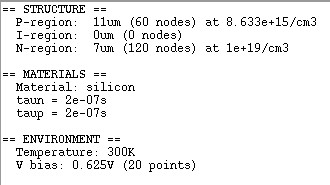
\includegraphics[width = 6cm]{inputs.jpg}
    \caption{Input Parameters in Simulator}
    \label{fig:inputs}
\end{figure}

\begin{figure}[!ht] 
    \centering
    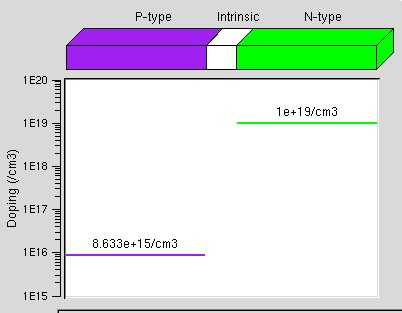
\includegraphics[width = 6cm]{doping.jpg}
    \caption{Doping Profile in Simulator}
    \label{fig:doping}
\end{figure}

\begin{figure}[!ht] 
    \centering
    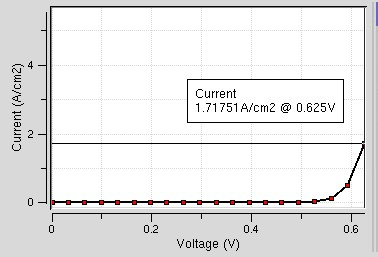
\includegraphics[width = 6cm]{current.jpg}
    \caption{IV-Characteristics in Simulator}
    \label{fig:current}
\end{figure}

\section*{Answers to Questions}

% REFERENCES!
\bibliographystyle{IEEEtran}
\bibliography{project3Bib.bib}

\end{document}
